\documentclass[12pt]{article}

\usepackage{geometry}
\usepackage{lmodern}
\usepackage{float}
\usepackage{fancyhdr}
\usepackage{amssymb}
\usepackage[linktocpage]{hyperref}
\usepackage{natbib}
\usepackage{xcolor}
\usepackage{parskip}
\usepackage{lastpage}
\usepackage{graphicx}
\usepackage{mhchem}
\usepackage{physics}
\usepackage{multirow}
\usepackage{xfrac}
\geometry{a4paper,left=1.5cm,right=1.5cm,top=2.5cm,bottom=2.5cm}

\fancyhf{}
\fancyhead[l]{Team \#15803}
\fancyhead[r]{Page \thepage\ of \pageref{LastPage}}
\pagestyle{fancy}
\setlength{\headheight}{15pt}

\newcommand{\identifierRedFont}[1]{{\huge \textbf{\textcolor{red}{#1}}}}
\newcommand{\todo}[1]{\textbf{[\textcolor{red}{TODO} #1]}}

\parskip=6pt

\begin{document}

\thispagestyle{empty}

\begin{center}
	Team Control Number
	
	\identifierRedFont{15803}

	Problem Chosen
	
	\identifierRedFont{B}

	\textbf{\large 2024} \\
	\textbf{HiMCM}

	\textbf{\small Summary Sheet}
\end{center}

\noindent\rule{\textwidth}{1pt}

\begin{center}
	\section*{Summary}
\end{center}

High-power computing (HPC) is becoming more and more popular in recent years due to the rising fame of artificial intelligence (AI) and cryptocurrencies. However, these technology advancements can actually cause severe harm to our environment. In this paper, we proposed an approach using math models to assess the environmental impacts due to HPC.

We first devised an \textbf{HPC energy consumption model}. We identified HPC activities into two sectors: HPC data centers and cryptocurrency mining. We estimated the energy consumption of data centers through country-wise working power data of all data centers and server utilization rates. We estimated the energy consumption of cryptocurrency mining through the total computing power of the whole network and the working efficiency of the current best mining machine. We then tested the accuracy of the modeled data and used them as a foundation throughout this paper.

We proposed the \textbf{HPC \ce{CO2} emission model} to identify the \ce{CO2} emissions from energy consumption data. We identified energy sources into three types: fossil fuels, nuclear energy, and renewable energy. We then calculated the country-wise energy mix and the per-energy carbon emission from available datasets. Combining these data with the energy consumption, we get the total carbon emission of HPC activities at a certain time. We then extended the model to a time series prediction. We separately modeled the trend of working power, total computing power of the whole network, working efficiency of the best mining machine, and changes in energy mix (country-wise). Using the model, we provided insights of the predicted data from now to the year of 2030. We also tested the cases of assuming to use half and all from renewable energy sources. We conducted a sensitivity analysis on the time-based model and discussed the results.

After that, we further expanded the model to a comprehensive \textbf{HPC environmental impact model}. We investigated the \ce{CO2} emissions in terms of the actual consequential global warming effects and proposed a set of qualitative measures to assess the severity of the emissions, with reference to the global warming control plan in the Paris Agreement. We also took another factor, the water usage, into consideration and developed a separate minor model to offer technical references.

According to the results of the comprehensive model, we designed a number of practical recommendations to reduce the environmental impacts, to policymakers and to tech companies and cryptocurrency miners, respectively. We also discussed the strengths and weaknesses of our models.

At the end of the paper, we wrote a letter to the United Nations Advisory Board, addressing that they did not include HPC's environmental impacts in their report on AI and urging them to include a detailed section with actionable plans in their 2030 development goals. We made use of our model and hoped to help shape a responsible future technological development.

\newpage

{\center\tableofcontents}

\newpage

\section{Introduction}

\subsection{Background information}

Under the current global trend of technology advancement, high-powered computing (HPC) is gaining rising attention for the increasing demand of computationally intensive tasks such as data science, artificial intelligence (AI) training, and cryptocurrency mining.

It is very common to use a massive number of dedicated hardware with strong computing power for these tasks. Data centers are the specific spaces to hold this hardware. The operation of data centers is usually extremely energy-consuming, with a tremendous demand of electricity to keep the computer systems running and to cool them down. They are forming a non-negligible sector of global energy consumption, taking up more than 1\% of the world's energy production \citep{IEA2024}. Cryptocurrency mining machine clusters also work similarly to data centers, with all resources dedicated for mining. The intensive use of electricity, contributing heavily to global warming, as well as a lot of other problems, e.g. water usage, e-waste, etc., poses the environmental concerns of HPC \citep{digiconomist}.

As sustainability arises as one of the most important development goals in the twenty-first century, it is high time we take action to assess the environmental consequences of HPC and to minimize its negative effects. We propose an approach to evaluate the environmental impacts due to HPC through mathematical models.

\subsection{Restatement of the problem}

In this paper, we divide the problems into the following tasks:
\begin{enumerate}
	\item We first devise an \textbf{HPC energy consumption model} as a foundation for our solution to the problem. We calculate the current annual energy consumption of each sector of HPC activities (data centers and cryptocurrency mining) by country. We will create two separate minor models to model the energy consumption of each sector.
	\item We then propose an \textbf{HPC \ce{CO2} emission model}. From available data of the energy mix of each country and the previously calculated country-wise HPC energy consumption, we can deduce the \ce{CO2} emission of HPC of each sector at present. After that, we model the trends of expansion of data centers, the expansion of cryptocurrency mining, and the change in energy mix over time separately. Combining these trends, we get the predictions of total \ce{CO2} emission till the year 2030. We will also test the effects of using 50\% of renewable sources and 100\% of renewable sources besides the case of the predicted energy mix.
	\item We also refine our model to take water consumption, as one more environmental factor other than \ce{CO2} emission, into consideration. This is to provide more realistic understandings of the \textbf{impact of HPC on the environment} and to better propose possible solutions. With the knowledge of the environmental impacts, we will then offer recommendations to firms and policy-makers to reduce the negative consequences.
\end{enumerate}

\section{HPC energy consumption model}

In this section, we model the annual worldwide energy consumption of \textit{high-powered computing} (HPC). HPC includes various computationally intensive tasks, which are mostly carried out by computer systems in data centers and cryptocurrency mining machines. Therefore, it is feasible to estimate the total energy consumption of HPC from these two sectors.

This model and data used will be the foundation for other models.

\subsection{Assumptions}
\label{sec_energy_model_assumptions}

\begin{enumerate}
	\item The total power data offered by data center providers reflects the maximum power. \\
	\textbf{Justification:} The data of total power in a data center is typically defined by the machines' design specifications. Therefore, we interpret this as the hard limit of the possible power allocated on the machines.
	
	\item Possible non-HPC data centers are also included. \\
	\textbf{Justification:} Since most data centers are hybrid, it is hard to exactly distinguish between HPC and non-HPC ones. Non-HPC hardware such as storage may also contribute to the process of HPC. Moreover, they share most of the infrastructure with HPC consuming a more significant amount of energy. Therefore, including some possible non-HPC facilities is not likely to create a large impact on the results.
	
	\item All data are from a same, \textit{short-run} scenario where there are no differences in conditions. \\
	\textbf{Justification:} Most of the data we found are statistics or information within or throughout the year 2022 to 2024. We tried to use the latest statistics, but this is not always available since the year of 2024 is not over yet by the time we work on this model. The assumption of the \textit{short-run} data means that we regard all data as taken from a same set of conditions with no development or changes between them; delving into the detailed differences would make the model way too complex and beyond the intended scope.

	\item The utilization rates across different data centers are the same. \\
	\textbf{Justification:} The actual utilization rates across different data centers are not varying very much. Since the emphasis of our model is on the estimation of total energy, the detailed utilization rates on each data center are not of significant interest and neglected.

	\item Bitcoin (BTC) mining is considered as the whole cryptocurrency mining industry. \\
	\textbf{Justification:} By the time we work on this model, Bitcoin (BTC) is the cryptocurrency with the largest capitalization and mining energy consumption. Cryptocurrencies other than BTC, namely \textit{altcoins}, consumes way less energy than BTC mining and could be negligible, especially with the second-largest Ethereum (ETH) switched to proof of stake (PoS) instead of the traditional proof of work (PoW) mining. \citep{digiconomist}

	\item Cryptocurrency mining machines are always operating at their \textit{full capacity rate}. \\
	\textbf{Justification:} As a highly-competitive industry, miners are profit-driven and tend to maximize their profits. Mining at the machines' full capacity ensures the maximum output which lowers the averaged fixed costs, such as the costs of mining machines and related infrastructures, and thus maximizes the profits.

	\item All other unlisted source of HPC are not considered. \\
	\textbf{Justification:} We believe the two sectors are enough to give a representation of all HPC activities. Unlisted sources, such as altcoin mining and small-scale server clusters, contributes very little on the total energy consumption.
\end{enumerate}

\subsection{Model overview}

\begin{table}[!t]
	\centering
	\caption{Definition of symbols. Units: TWh: terawatt hours; MW: megawatts; TH: terahashes.}
	\label{table_symbols_q1}
	\begin{tabular}{lll}
		\hline
		\textbf{Symbol} & \textbf{Unit} & \textbf{Description} \\
		\hline
		$E$ & TWh & Total annual energy consumption of all HPC activities. \\
		$E_D$ & TWh & Total annual energy consumption of data centers. \\
		$E_M$ & TWh & Total annual energy consumption of cryptocurrency mining. \\
		$T$ & h & The time duration (in this case, $\rm = 1yr = 8760h$). \\
		$P_i$ & MW & Total maximum power of data center $i$. \\
		$\overline{\rho}$ & -- & Average utilization rate of data centers. \\
		$H$ & TH/s & Total hash rate performed by the network. \\
		$\kappa$ & -- & Multiplier between the average and the optimal mining efficiency. \\
		$\varepsilon_{\rm opt}$ & J/TH & Efficiency of the best mining machine (power per hash rate). \\
		$\overline{\varepsilon}$ & J/TH & Average efficiency among mining machines ($\overline{\varepsilon} = \kappa \varepsilon_{\rm opt}$). \\
		\hline
	\end{tabular}
\end{table}

We define a set of symbols as in Table \ref{table_symbols_q1}. The total annual power consumption of HPC is
\begin{equation}
	E = E_D + E_M,
\end{equation}
which is the sum of energy consumed by data centers and cryptocurrency mining. In this model, some proportional relationships will be intentionally introduced to facilitate the subsequent models.

\subsubsection{Energy consumption of data centers}

The annual energy consumption of data centers \textit{at full capacity} is straightforwardly defined as
\begin{equation}
	E_{D \rm max} = T \sum_i P_i,
\end{equation}
which is the product of the time of a year and the sum of maximum powers of all data centers. To get the case at \textit{average utilization rate}, we simply multiply it by the average utilization rate $\overline{\rho}$:
\begin{equation}
	E_{D \rm avg} = \overline{\rho} E_{D \rm max} = \overline{\rho} T \sum_i P_i.
\end{equation}

\subsubsection{Energy consumption of cryptocurrency mining}

During cryptocurrency mining, many miners join a network to solve blocks. The \textit{hash rate} is a measure of the computational power of a machine, defined as the number of hash calculations performed per unit time. The total hash rate $H$ of a network is the sum of the hash rates of all machines connected to the network, with a higher value representing a higher competition among miners.

A mining machine works at a specific power and holds a specific computational power, or hash rate. The ratio between the working power and its computational power gives its \textit{efficiency} $\varepsilon$, the power required to achieve unit hash rate (in the unit of power per hash rate, or energy per hash).

To calculate the total power $P$ in a network, we multiply the average efficiency $\overline{\varepsilon}$ among all mining machines with the network's total hash rate $H$ \citep{btc_energy}:
\begin{equation}
	P = \overline{\varepsilon} H.
	\label{eq_mining_power}
\end{equation}

Over time, new mining machines with more advanced technologies are produced and slowly take up the market whilst old machines are still being used (economically speaking, they will be used until their outputs are lower than their operating costs). Therefore, the replacement process takes time; the average efficiency is always lower than the efficiency of the latest machine.

We define $\kappa$ as the ratio between the average efficiency $\overline{\varepsilon}$ (among all machines) and the optimal efficiency $\varepsilon_{\rm opt}$ (of the current best model). Equation \ref{eq_mining_power} can be rewritten as
\begin{equation}
	P = \overline{\varepsilon} H = \kappa \varepsilon_{\rm opt} H.
\end{equation}

Finally, we multiply the power with the one-year time $T$ to get the annual energy consumption:
\begin{equation}
	E_M = PT = \kappa \varepsilon_{\rm opt} HT;
	\label{eq_crypto_energy}
\end{equation}
this is both the \textit{full capacity} level and the \textit{average utilization} level since cryptocurrency mining is assumed to be always operating at the maximum utilization possible.

\subsubsection{Total annual energy consumption}

Combining the above equations, the total annual energy consumption at \textit{full capacity} is expressed as
\begin{equation}
	E_{\rm max} = E_{D \rm max} + E_M = T \sum_i P_i + \kappa \varepsilon_{\rm opt} HT,
\end{equation}
and the total annual energy consumption at \textit{average utilization rate} is
\begin{equation}
	E_{\rm avg} = E_{D \rm avg} + E_M = \overline{\rho} T \sum_i P_i + \kappa \varepsilon_{\rm opt} HT.
\end{equation}

\subsection{Assessing the model using current data}

To assess the accuracy of the energy consumption model, we substitute existing data into our model and compare the model's output with the related existing aggregated statistics.

\subsubsection{Data centers}

We acquired data from \textit{datacenters.com}, a website offering detailed information of data centers worldwide. 4342 data centers \citep{datacenters_com} are included, with information of each's name, location, provider, space, total power, etc. Table \ref{table_data_datacenters.com} shows some of the results from the website.

\begin{table}[!t]
	\centering
	\caption{Some records of data center information from \textit{datacenters.com}. Only columns including data related to the model are displayed; names and addresses that are too long are truncated.}
	\label{table_data_datacenters.com}
	\small
	\begin{tabular}{clrrr}
		\hline
		\textbf{ID} & \textbf{Name} & \textbf{Address} & \textbf{Total space} (sqft) & \textbf{Total power} (MW) \\
		\hline
		0 & Equinix: ... & ..., Tokyo, Japan & 58992 & 6.75 \\
		1 & KAO Data: ... & ..., UK & 40000 & 40 \\
		2 & NorthC: Eindhoven ... & ..., Netherlands & 43056 & 4.5 \\
		3 & DC2Scale: ... & ..., France & 15000 & 1.5 \\
		4 & DataBank: ... & ..., TX, USA & 23000 & 0.675 \\
		5 & Digital Realty: ... & ..., Opfikon, Switzerland & 79800 & 5 \\
		6 & Ascenty, ... & ..., São Paulo, Brazil & 22604.21 & 34 \\
		7 & EdgeConnex: ... & ..., Calle Larga, Chile & 116519.33 & 14 \\
		8 & Centersquare: ... & ..., MA, USA & 201590 & 15 \\
		9 & Digital Realty: ... & ..., Tamil Nadu, India & 196000 & 20.4 \\
		$\vdots$ &&&& \\
		4341 & Equinix: ... & ..., São Paulo, Brazil & 52743 & 1.8 \\
		\hline
	\end{tabular}
\end{table}

We plotted the distribution of the data as in Figure \ref{fig_data_datacenters_original}; it is worth mentioning that there are two very significant outlier values (denoted yellow on the top) exceeding $10^6$ megawatts. Obviously, it is improbable for those two data centers to consume about 13 times more power than the sum of all other ones (more intuitively, taking up almost 5\% of the total human power consumption); therefore, the data is very possibly incorrectly recorded or in a wrong unit. We thereby removed the two, and now all data are in a reasonable range, as shown in Figure \ref{fig_data_datacenters_clean}.

\begin{figure}[!t]
	\centering
	\begin{minipage}{0.48\textwidth}
		\centering
		\label{fig_data_datacenters_original}
		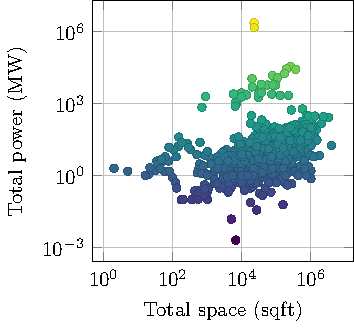
\includegraphics{figures/data/datacenters.pdf}
		\caption{The original dataset.}
	\end{minipage}
	\begin{minipage}{0.48\textwidth}
		\centering
		\label{fig_data_datacenters_clean}
		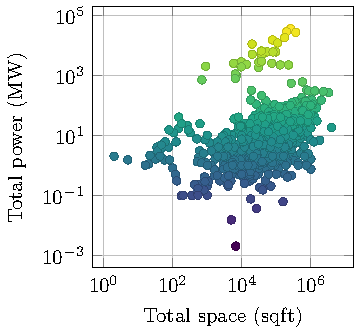
\includegraphics{figures/data/datacenters_clean.pdf}
		\caption{The dataset with outliers removed.}
	\end{minipage}
\end{figure}

We then calculated the sum of the total powers of all data centers without the outliers, yielding $\sum_i P_i = 309,160 \rm MW$. Therefore, the annual energy consumption of data centers at \textit{full capacity} is
\begin{equation}
	E_{D \rm max} = T \sum_i P_i =
	\rm 8,760h \times 309,160MW \approx \mathbf{2,708TWh}.
\end{equation}

The 2024 Kubernetes Cost Benchmark Report \citep{kubernetes_report} reveals that the average utilization rate for Kubernetes server clusters is 13\%. Since Kubernetes is widely used in data centers, this figure is highly representative for general data center utilization. Therefore, we get the annual energy consumption of data centers at \textit{average utilization rate}:
\begin{equation}
	E_{D \rm avg} = \overline{\rho} E_{D \rm max}
	= \rm 13\% \times 2,708TWh \approx \mathbf{352TWh}.
\end{equation}

This falls in the range of energy consumption estimated by the International Energy Agency (IEA), that data centers consume have a total annual energy consumption between 240TWh and 340TWh \citep{IEA2024}.

\subsubsection{Cryptocurrency mining}

Using the recent (November 2024) Bitcoin network data \citep{hashrate}, the total hash rate $H \approx \rm 750,000,000TH/s$. The currently most advanced mining machine is Antminer S21 \citep{best_miner}, with required power of 3531W and a hash rate of 300TH/s, giving the efficiency
\begin{equation}
	\varepsilon_{\rm opt} = \rm \frac{3531W}{300TH/s} = 11.77J/TH.
\end{equation}

According to an examination of a real-world mine \citep{miner_avg_eff}, the actual power consumption of the mine is about 70\% higher than the theoretical optimum, thus the multiplier $\kappa = 1.7$. This gives the total annual energy consumption of cryptocurrency mining:
\begin{equation}
	E_M = \kappa \varepsilon_{\rm opt} HT
	= \rm 1.7 \times 11.77J/TH \times 750,000,000TH/s \times 8,760h \approx \mathbf{131TWh},
\end{equation}
which also falls in the range of the estimated data of Bitcoin mining energy consumption for the year of 2024 \citep{digiconomist}, between 124TWh and 175TWh.

\subsubsection{Evaluation}

Combining the results, the total annual energy consumed by all HPC activities is $352 + 131 = 483 \rm TWh$. This data falls in a realistic boundary per current statistics and is highly reliable.

\section{HPC carbon dioxide emission model}

In this section, we model the \ce{CO2} emissions of all HPC activities based on the previous energy consumption model. We will first present the model at a fixed time, and then take the time variance into consideration. We additionally define several symbols in this model, as shown in Table \ref{table_symbols_q2}.

\subsection{Assumptions}

Assumptions in Section \ref{sec_energy_model_assumptions} are still used in this section. Here are the additional assumptions:

\begin{enumerate}
	\item The energy mix of a data center is exactly the same as the energy mix of the country it is in. \\
	\textbf{Justification:} Most data centers are directly connected to the national electrical grid, which's electricity comes from a mixed source. The detailed investigation of the energy mix at each location is far beyond the scope of this model; we hence simplify this to a uniform national averaged distribution of electricity source.

	\item All data, such as total power and energy mix, are discretized for each year, i.e., within one year, the data is uniform and does not change. \\
	\textbf{Justification:} This assumption is to match most of the data that comes in the form of annual statistics. Since the model aims to provide insights on the current state and long-term future predictions of \ce{CO2} emissions, ignoring the temporal variations within one year simplifies the model and makes it easier to be implemented from data.

	\item Each type of energy source has a same fixed \ce{CO2} emission per unit energy in every country and does not change over time. \\
	\textbf{Justification:} In reality, a same type of energy source may have different \ce{CO2} emissions in different places (e.g., the difference in the effectiveness of wind power due to different natural conditions at different sites); technological advancements also reduces \ce{CO2} emissions (e.g., by increasing the efficiency of resource usages). To accurately model these, we would need time-varying emissions data at province level or even city level; such differences are ignored because they would make the model too complex while not creating any significant change.

	\item The HPC industry is an ever-developing industry throughout the timeframe we are modeling. \\
	\textbf{Justification:} It is impossible to determine whether, why and when the industry will continue to expand, mature and stagnate, or decay in the future. Since past data of HPC shows its consistent growth in the past years, and we are investigating its development over a medium time span (compared with the time range of available data), it is reasonable for us to assume the persistence of this trend and simplify the model.

	\item The \ce{CO2} emissions during the production and disposal of computer systems or related infrastructures are not counted as HPC emissions. \\
	\textbf{Justification:} It is hard to determine whether and by how much are this hardware related to HPC. In addition, it would make the model extremely complicated to calculate the carbon emission data of a range of types of hardware. Therefore, they are not included in the model we propose, and only operational carbon emissions are calculated.
\end{enumerate}

\begin{table}[!t]
	\centering
	\caption{Definition of new symbols. The symbol $x \in \left\{ \rm F, N, R \right\}$ stands for the method of electricity production, respectively fossil fuels (F), nuclear energy (N), and renewable energy (R).}
	\label{table_symbols_q2}
	\begin{tabular}{lll}
		\hline
		\textbf{Symbol} & \textbf{Unit} & \textbf{Description} \\
		\hline
		$\Psi$ & t & Total annual \ce{CO2} emission of all HPC activities. \\
		$\Psi_D$ & t & Total annual \ce{CO2} emission of data centers. \\
		$\Psi_M$ & t & Total annual \ce{CO2} emission of cryptocurrency mining. \\
		$\Xi_{i,\rm T}$ & TWh & Total annual electricity production of country $i$. \\
		$\Xi_{i,x}$ & TWh & Annual electricity production of country $i$ using method $x$. \\
		$M_{x}$ & t/TWh & Mass of \ce{CO2} created per unit of electricity produced using method $x$. \\
		$C_{i}$ & t/TWh & \ce{CO2} emission per unit electricity produced in country $i$. \\
		$\zeta_{i,x}$ & -- & Proportion of electricity production of country $i$ using method $x$. \\
		$\zeta_{{\rm M},x}$ & -- & Proportion of electricity for crypto. mining produced using method $x$. \\
		$t$ & -- & A particular year in A.D. \\
		\hline
	\end{tabular}
\end{table}

\subsection{Carbon dioxide emissions at a fixed time (present)}

Similarly, we calculate the total emissions through adding up the two sectors. We categorize all energy sources that are used to produce electricity into three types: fossil fuels (F), nuclear energy (N), and renewable energy (R). In this section, all calculations will use the current data.

\subsubsection{Carbon dioxide emission of data centers}

Suppose the electricity production of country $i$ (with a total of $n$ countries) from energy type $x$ is $\Xi_{i,x}$, we have the mix and total energy for the production of electricity of all countries:
\begin{equation}
	\vb{\Xi} = \begin{bmatrix}
		\Xi_{1,\rm F} & \Xi_{1,\rm N} & \Xi_{1,\rm R} \\
		\Xi_{2,\rm F} & \Xi_{2,\rm N} & \Xi_{2,\rm R} \\
		\vdots & \vdots & \vdots \\
		\Xi_{n,\rm F} & \Xi_{n,\rm N} & \Xi_{n,\rm R} \\
	\end{bmatrix}; \quad
	\vb{\Xi_T}
	= \begin{bmatrix}
		\Xi_{1,\rm T} \\
		\Xi_{2,\rm T} \\
		\vdots \\
		\Xi_{n,\rm T} \\
	\end{bmatrix}
	= \begin{bmatrix}
		\Xi_{1,\rm F} + \Xi_{1,\rm N} + \Xi_{1,\rm R} \\
		\Xi_{2,\rm F} + \Xi_{2,\rm N} + \Xi_{2,\rm R} \\
		\vdots \\
		\Xi_{n,\rm F} + \Xi_{n,\rm N} + \Xi_{n,\rm R} \\
	\end{bmatrix}
	= \vb{\Xi} \vb{1}.
\end{equation}

Therefore, we define the proportions of the electricity produced from each energy source in all electricity production for each country, $\boldsymbol{\zeta} \in \mathbb{R}^{n \times 3}$, as
\begin{equation}
	\zeta_{i, x}
	= \frac{\Xi_{i, x}}{\Xi_{i,\rm T}}
	= \frac{\Xi_{i, x}}{\Xi_{i,\rm F} + \Xi_{i,\rm N} + \Xi_{i,\rm R}}, \quad
	\left(
		x \in \left\{ \rm F, N, R \right\}
	\right).
\end{equation}

For the mass of \ce{CO2} created per unit of electricity
\begin{equation}
	\vb{M} = \begin{bmatrix}
		M_{\rm F} \\
		M_{\rm N} \\
		M_{\rm R} \\
	\end{bmatrix},
\end{equation}
the energy mix proportions $\boldsymbol{\zeta}$ are the weights on each energy type; through linear combination, we calculate the weighted average \ce{CO2} emission per unit electricity in each country as
\begin{equation}
	\vb{C} = \boldsymbol{\zeta} \vb{M}.
\end{equation}

Since we already have the detailed information of all data centers, we can calculate the total capacity power of data centers in each country as
\begin{equation}
	\vb{P} = \begin{bmatrix}
		\sum_{P_i \rm\;in\;country\;1} P_i \\
		\sum_{P_i \rm\;in\;country\;2} P_i \\
		\vdots \\
		\sum_{P_i \rm\;in\;country\;n} P_i \\
	\end{bmatrix},
\end{equation}
giving the total \textit{real} energy consumption due to data centers in each country
\begin{equation}
	\vb{E_D} = \overline{\rho} T \vb{P},
\end{equation}
where $\overline{\rho}$ is the average utilization rate and $T$ is the time period (one year).

Through linear combination, we deduce the total annual \ce{CO2} emissions worldwide due to data centers by calculating the multiplication of annual energy and \ce{CO2} emission per energy:
\begin{equation}
	\Psi_D = \vb{E_D}^\top \vb{C} = \overline{\rho} T \vb{P}^\top \boldsymbol{\zeta} \vb{M}.
	\label{eq_dc_emission}
\end{equation}

\subsubsection{Carbon dioxide emission of cryptocurrency mining}

The industry of cryptocurrency mining is separated mainly for the difficulty in identifying country-wise energy mix. However, the energy mix of the industry as a whole is feasible. We could model the industry in a way similar to modeling another country.

Previously, we have calculated that the annual energy consumption because of cryptocurrency mining is $E_M = \kappa \varepsilon_{\rm opt} HT$. Similarly, we can calculate the \ce{CO2} emission per unit of electricity as
\begin{equation}
	\vb{C_M} = \boldsymbol{\rm \zeta_M} \vb{M}, \quad
	\left(
		\boldsymbol{\rm \zeta_M} =
		\begin{bmatrix}
			\zeta_{\rm M, F} & \zeta_{\rm M, N} & \zeta_{\rm M, R} \\
		\end{bmatrix}
	\right),
\end{equation}
and therefore, the total \ce{CO2} emission due to cryptocurrency mining can be defined:
\begin{equation}
	\Psi_M = E_M \vb{C_M} = \kappa \varepsilon_{\rm opt} HT \boldsymbol{\rm \zeta_M} \vb{M}.
\end{equation}

\subsubsection{Results and evaluation}

We add up the two sectors to find the total annual \ce{CO2} emission of HPC:
\begin{equation}
	\Psi = \Psi_D + \Psi_M
	= \overline{\rho} T \vb{P}^\top \boldsymbol{\zeta} \vb{M}
		+ \kappa \varepsilon_{\rm opt} HT \boldsymbol{\rm \zeta_M} \vb{M}.
\end{equation}

We use the World Energy Balances 2024 Highlights (free extract) dataset \citep{energy_mix_dataset} offered by the International Energy Agency (IEA). The dataset includes comprehensive energy mix data over the past fifty years (since 1971) in many countries and broader regions, including total electricity production and production from fossil fuels, nuclear energy, and renewable energy, as exampled in Table \ref{table_iea_energy_dataset}. Figure \ref{fig_emission_data_availability} shows the most accurate data available from the dataset for each country. Countries having the most data centers, such as the U.S., western European countries, China, Japan, Singapore, etc., all have their own country-specific data available. Therefore, the dataset is highly reliable for modeling the energy structure used by data centers worldwide.

\begin{figure}[!t]
	\centering
	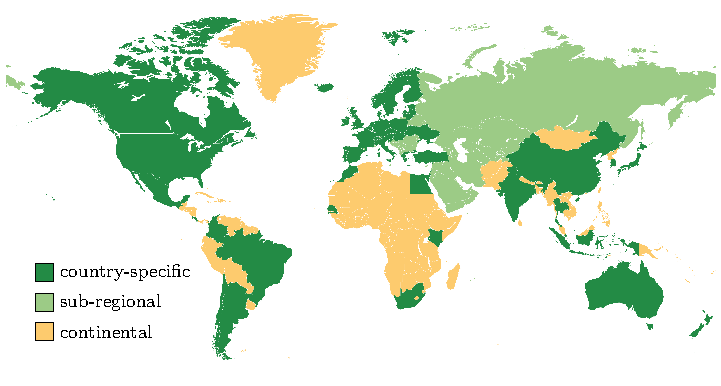
\includegraphics{figures/data/emission_map.pdf}
	\vspace*{-0.5cm}
	\caption{Detailed energy mix data availability in each country.}
	\label{fig_emission_data_availability}
\end{figure}

\begin{table}[!t]
	\centering
	\caption{An extract from the IEA World Energy Balances 2024 Highlights dataset.}
	\label{table_iea_energy_dataset}
	\small
	\begin{tabular}{cllrrrrr}
		\hline
		\multirow{2}*{\textbf{Entry}} & \multirow{2}*{\textbf{Country}} & \multirow{2}*{\textbf{Energy Type}} & \multicolumn{5}{c}{\textbf{Electricity output} (GWh)} \\
		&&& \textbf{1971} & \textbf{1972} & $\cdots$ & \textbf{2022} & $\mathbf{2023}^{\dagger}$ \\
		\hline
		1 & Australia & Fossil fuels & 41201 & 43730 & $\cdots$ & 187536 & 181363 \\
		2 & Australia & Nuclear & 0 & 0 & $\cdots$ & 0 & 0 \\
		3 & Australia & Renewable sources & 11844 & 11853 & $\cdots$ & 83282 & 92216 \\
		4 & Australia & Total & 53045 & 55583 & $\cdots$ & 270818 & 273579 \\
		5 & Austria & Fossil fuels & 11752 & 11939 & $\cdots$ & 13509 & 10205 \\
		6 & Austria & Nuclear & 0 & 0 & $\cdots$ & 0 & 0 \\
		7 & Austria & Renewable sources & 16450 & 16986 & $\cdots$ & 50432 & 59397 \\
		8 & Austria & Total & 28202 & 28925 & $\cdots$ & 64713 & 70301 \\
		$\vdots$ \\
		244 & World & Total & 5256947 & 5698376 & $\cdots$ & 29143442 & -- \\
		\hline
	\end{tabular}
\end{table}

We acquired data for power sector emissions worldwide from Ember \citep{emission_dataset}, including \ce{CO2} emissions due to coal, gas, other fossil, bioenergy, hydro, solar, wind, nuclear, and other renewables, from the year 2000 to 2023. We extracted the data of 2022: 13,665.56Mt from fossil fuels, 13.61Mt from nuclear energy, and 338.61Mt from renewable energies.

Using data from IEA, we know that in 2022 the world produced 17,772,682GWh, 2,685,464GWh, and 8,559,418GWh, respectively, from the three sources. By dividing the emission with the electricity produced, we get the \ce{CO2} emission created per unit of electricity in 2022 (in t/TWh):
\begin{equation}
	\vb{M} = \begin{bmatrix}
		768,908 \\ 5,068 \\ 39,560
	\end{bmatrix}.
\end{equation}

Taking all these data, we have
\begin{equation}
	\Psi_D
	= \overline{\rho} T \vb{P}^\top \boldsymbol{\zeta} \vb{M}
	= 13\% \times 1 {\rm yr} \times 0.130 {\rm Mt/h} = 148 {\rm Mt}
\end{equation}
\ce{CO2} (Mt: million tons) emitted due to data centers.

\begin{figure}[!t]
	\centering
	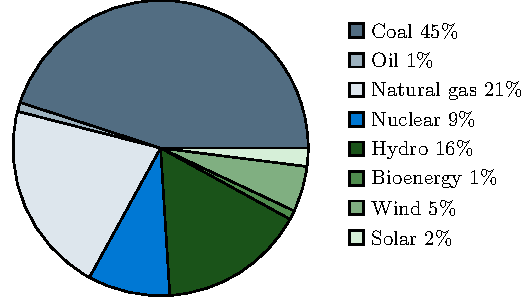
\includegraphics{figures/data/bitcoin_mix.pdf}
	\caption{Energy mix of Bitcoin mining.}
	\label{fig_bitcoin_mix}
\end{figure}

The energy mix used to supply Bitcoin mining is shown in Figure \ref{fig_bitcoin_mix} \citep{bitcoin_mix}. The energy consumption of the industry is 67\% from fossil fuels, 9\% from nuclear energy, and 24\% from renewable sources. Therefore, we calculate the \ce{CO2} emission of cryptocurrency mining as
\begin{equation}
	\Psi_M = E_M \boldsymbol{\rm \zeta_M} \vb{M}
	= 131 {\rm TWh} \cdot \begin{bmatrix}
		0.67 & 0.09 & 0.24
	\end{bmatrix}\begin{bmatrix}
		768,908 \\ 5,068 \\ 39,560
	\end{bmatrix} {\rm t/TWh}
	= 68.8 {\rm Mt};
\end{equation}
hence, the total \ce{CO2} emission of HPC at present is
\begin{equation}
	\Psi = \Psi_D + \Psi_M = 148 + 68.8 = 216.8 {\rm Mt}.
\end{equation}

\subsection{Change in carbon dioxide emission over time}

Previously, we calculated the \ce{CO2} emissions created by HPC at present from several components. By modeling the trends of these components' changes over time, we will construct a model for the future predictions.

\subsubsection{Modeling the change of data centers}

Google is one of the largest firms dominating the market of HPC data centers. We consider it as a reliable representative of the whole industry.

From Google 2024 Environmental Report \citep{google_report}, we have Google's annual energy consumption from 2011 to 2023. The data is plotted in Figure \ref{fig_google} (left). Energy consumption is directly related to the expansion of the industry. From the graph, we can identify an increasing rate of increment in annual energy consumption. This is typically defined by an exponential relationship where there is a constant rate of increasing proportion, i.e., constant ratio between two consecutive years.

\begin{figure}[!t]
	\centering
	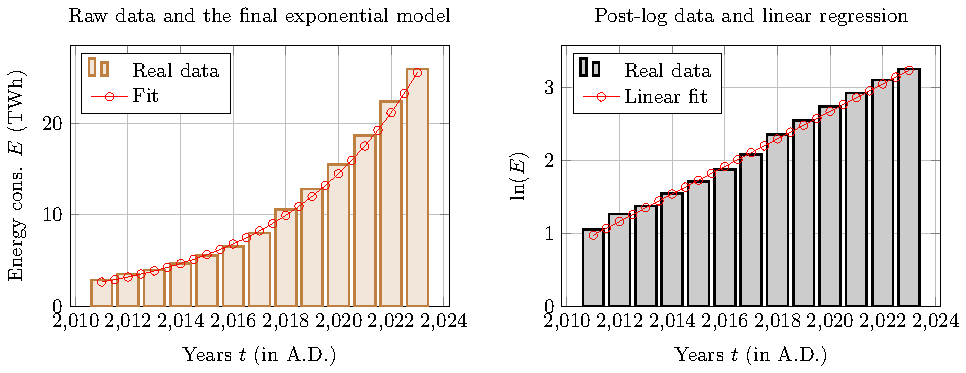
\includegraphics{figures/trends/google.pdf}
	\caption{Trend of Google's annual energy consumption from financial year 2011 to 2023. \textbf{Left:} the real data and the exponential fit deduced from the linear fit of the post-log data on the right side. \textbf{Right:} data normalized using natural logarithm and the linear regression on the processed data.}
	\label{fig_google}
\end{figure}

We thereby calculate the natural logarithm of each data to linearize the trend, as shown in Figure \ref{fig_google} (right). It is obvious that the data is now almost perfectly following a linear trend; therefore, the exponential relationship exists and is a proper way to model the change. Through linear regression (having a correlation of $r \approx 0.99$), we have
\begin{equation}
	\ln \left(E(t)\right) = 0.1887t - 378.5;
\end{equation}
therefore,
\begin{equation}
	E(t) = \exp \left(0.1887t - 378.5\right) = 4.1643 \times 10^{-165} \cdot \exp \left(0.1887t\right).
\end{equation}

Thus, we can calculate the annual increment multiplier $r$ as
\begin{equation}
	r = \frac{E\left(t + 1\right)}{E(t)}
	= \frac{\exp \left(0.1887\left(t + 1\right) - 378.5\right)}{\exp \left(0.1887t - 378.5\right)}
	= \exp \left(0.1887\right).
\end{equation}

Using the previously calculated data of current (2024) global energy consumption of 352TWh from HPC data centers, we can model that
\begin{equation}
	\begin{aligned}
		E_D(t) &= E_D(2024) \cdot r^{t - 2024} = 352 \cdot \exp \left(0.1887(t - 2024)\right) \\
		&= 4.7531 \times 10^{-164} \cdot \exp \left(0.1887t\right),
	\end{aligned}
\end{equation}
for any year $t$. Figure \ref{fig_energy_datacenter} shows the calculated numerical values.

\begin{figure}[!t]
	\centering
	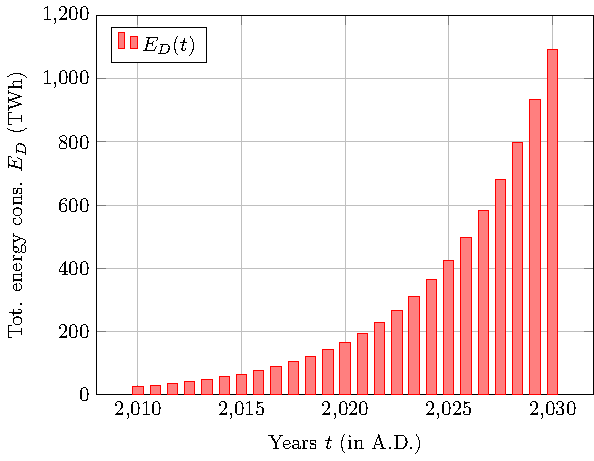
\includegraphics{figures/trends/datacenter_energy.pdf}
	\caption{Estimated energy consumption due to HPC data centers.}
	\label{fig_energy_datacenter}
\end{figure}

\subsubsection{Modeling the change of cryptocurrency mining}

As deduced in Equation \ref{eq_crypto_energy}, $E_M = \kappa \varepsilon_{\rm opt} HT$. We assume the ratio $\kappa$ to be constant over time. Since our model will be mostly applied to a medium timeframe, $\kappa$, mainly dependent on the distribution of hardware types, are not likely to fluctuate rapidly as the best efficiency of hardware $\varepsilon_{\rm opt}$ or the total hash rate $H$. We thereby model the change in $\varepsilon_{\rm opt}$ and $H$ over time $t$ respectively.

To investigate the trend of the development of the most energy-efficient cryptocurrency mining machine, we aggregated the various lists of data of all mining machines from a range of hardware vendors, researches, and online cryptocurrency-related databases, for the year of 2015 \citep{best_miner_2015}, 2017 \citep{btc_energy}, 2021 \citep{best_miner_2021}, 2022 \citep{best_miner_2022}, 2023 \citep{best_miner_2023}, and 2024 \citep{best_miner}. The extracted data of the miners with the best (smallest) efficiency, which is defined as $\varepsilon = P / H$, is presented in Table \ref{table_best_miners}.

\begin{table}[!t]
	\centering
	\caption{List of the best cryptocurrency mining machine: powers, hash rates, and efficiencies.}
	\label{table_best_miners}
	\small
	\begin{tabular}{c|lrr|r}
		\hline
		\textbf{Year} & \textbf{Model} & $\boldsymbol{P}$ (W) & $\boldsymbol{H}$ (TH/s) & $\boldsymbol{\varepsilon}$ (J/TH)\\
		\hline
		2015 & Antminer S7 & 1,293 & 4.73 & 273.4 \\
		2017 & Antminer S9 & 1,372 & 14 & 98.0 \\
		2021 & Antminer S19 Pro & 3,250 & 110 & 29.5 \\
		2022 & Antminer S19 XP & 3,010 & 140 & 21.5 \\
		2023 & Antminer S19 XP Hyd & 5,304 & 255 & 20.8 \\
		2024 & Antminer S21 & 3,531 & 300 & 11.8 \\
		\hline
	\end{tabular}
\end{table}

\begin{figure}[!t]
	\centering
	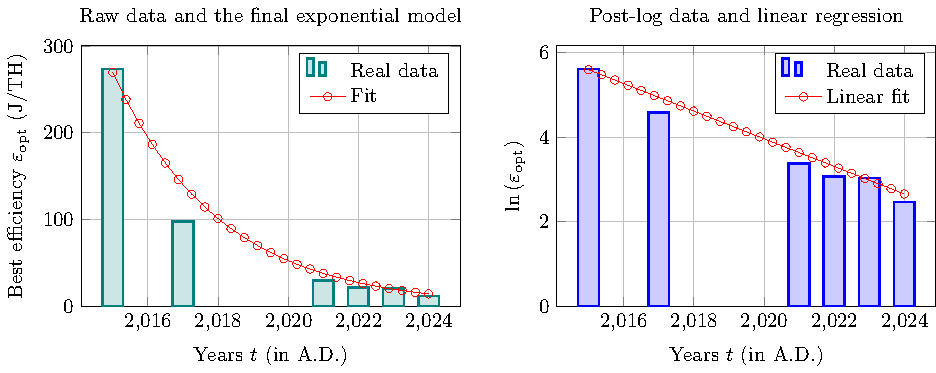
\includegraphics{figures/trends/miner.pdf}
	\caption{The trend of cryptocurrency miner's best efficiency $\varepsilon_{\rm opt}$ over years. \textbf{Left:} the real data and the exponential fit calculated from the linear fit result of post-log data on the right side. \textbf{Right:} data normalized using natural logarithm with the consequential linear fit on post-log data.}
	\label{fig_miner_trend}
\end{figure}

As illustrated in the Green500 list from the TOP500 list of supercomputers \citep{top500}, the growth of computational performance per power consumed is exponential. The efficiency $\varepsilon$ defined in this research, which is the ratio of power to hash rate, is the reciprocal of the performance per power; this makes $1/\varepsilon_{\rm opt}$ have an exponential growth over time, i.e., $\varepsilon_{\rm opt}$ would decay exponentially over time (since $1/e^x = e^{-x}$).

A straightforward approach to model the exponential relationship would be linearization of the data. We take the natural logarithm values of the efficiencies, $\ln\left(\varepsilon_{\rm opt}\right)$, and find its relationship with the time $t$, as shown in Figure \ref{fig_miner_trend}. Through linear regression, we get
\begin{equation}
	\ln\left(\varepsilon_{\rm opt} (t)\right) = -0.3268t + 664.1,
\end{equation}
with a correlation of $r \approx -0.99$, and hence the efficiency can be modeled as
\begin{align}
	\varepsilon_{\rm opt} (t) = \exp \left(-0.3268t + 664.1\right)
	&= 2.6 \times 10^{288} \cdot \exp \left(-0.3268t\right) {\rm J/TH} \\
	&= 2.6 \times 10^{276} \cdot \exp \left(-0.3268t\right) {\rm TJ/TH}.
	\label{eq_efficiency}
\end{align}

The Bitcoin network's total hash rate data \citep{hashrate} is plotted in Figure \ref{fig_total_hashrate}, starting from January 2009, the time when Bitcoin was created. The total hash rate increases with faster rates over time. Despite having small fluctuations, the pattern should follow either an exponential model (constantly increasing proportion) or a power function model (growth with limiting resources).

\begin{figure}[!t]
	\centering
	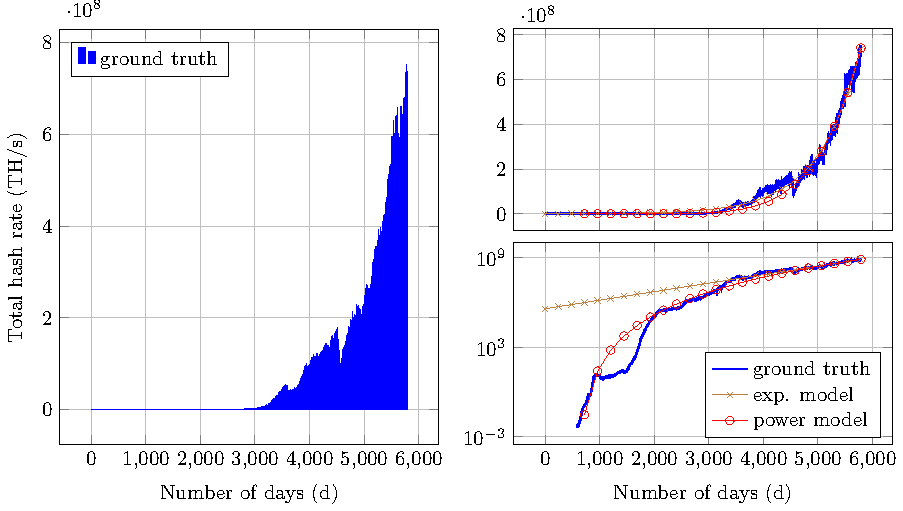
\includegraphics{figures/trends/bitcoin_hashrate.pdf}
	\caption{Total hash rate of the Bitcoin network over time and comparison across models. January 10, 2009, is selected as the day 0. \textbf{Left:} the ground truth. \textbf{Right:} comparison between the exponential model and the power function model, displayed in linear axis (top) and log scaled axis (bottom).}
	\label{fig_total_hashrate}
\end{figure}

From Figure \ref{fig_total_hashrate} (right), we see that both the exponential model and the power function model showcase a decent capture of the trend (both with a correlation $r \approx 0.99$). However, when the models are compared within a log scaled $y$-axis, the data actually ``bends'' and does not follow a constantly increasing magnitude. The exponential model has deviations with the data trend, whereas the power function almost perfectly matches the data. Therefore, it can be concluded that the total hash rate follows the model
\begin{equation}
	H = 3.087 \times 10^{-16} \cdot (x - 588)^{6.561} \rm TH/s,
\end{equation}
where $x$ is the number of days starting from January 10, 2009. Convert $x$ to years $t$ (A.D.) assuming 365 days every year: $t = 2009 + \frac{1}{365}(x + 10) \Rightarrow x = 365 t - 733295$. Therefore,
\begin{equation}
	H(t) = 19.9867 \left( t - 2,010.6384 \right)^{6.561} \rm TH/s.
	\label{eq_hash_rate}
\end{equation}

Combining Equation \ref{eq_efficiency} for $\varepsilon_{\rm opt} (t)$ and Equation \ref{eq_hash_rate} for $H(t)$, we get the model for the total energy consumed by cryptocurrency mining over time:
\begin{equation}
	\begin{aligned}
		E_M (t) &= \kappa \varepsilon_{\rm opt} (t) H(t) T \\
		&= 1.7 \cdot \left(
			2.6 \times 10^{276} \cdot \exp \left(-0.3268t\right) {\rm TJ/TH}
		\right) \cdot \left(
			19.9867 \left( t - 2,010.6384 \right)^{6.561} {\rm TH/s}
		\right) \cdot 8,760 {\rm h} \\
		&= 7.7387 \times 10^{281} \cdot \exp \left(-0.3268t\right) \cdot \left( t - 2,010.6384 \right)^{6.561} {\rm TWh},
	\end{aligned}
\end{equation}
for a given year $t$. The calculated numerical values of this model are shown in Figure \ref{fig_crypto_energy_pred}.

\begin{figure}[!t]
	\centering
	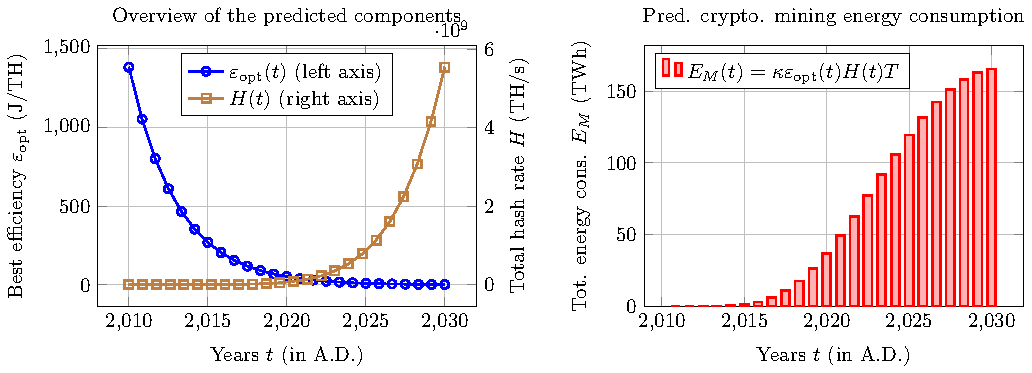
\includegraphics{figures/trends/crypto_energy.pdf}
	\caption{Numerical values of the model from year 2010 to 2030. \textbf{Left:} the values of the predicted components $\varepsilon_{\rm opt}(t)$ and $H(t)$. \textbf{Right:} the estimated total energy consumption of each year.}
	\label{fig_crypto_energy_pred}
\end{figure}

\subsubsection{The effects of change in energy mix}

Previously, we calculated the energy mix of each country $\boldsymbol{\zeta}$ from the dataset offered by IEA. These values also vary over time. We plot an extract of the trends of some countries and sub-regions in Figure \ref{fig_mix_data}. The changes in proportions of the three energy sources all follow a linear relationship.

\begin{figure}[!t]
	\centering
	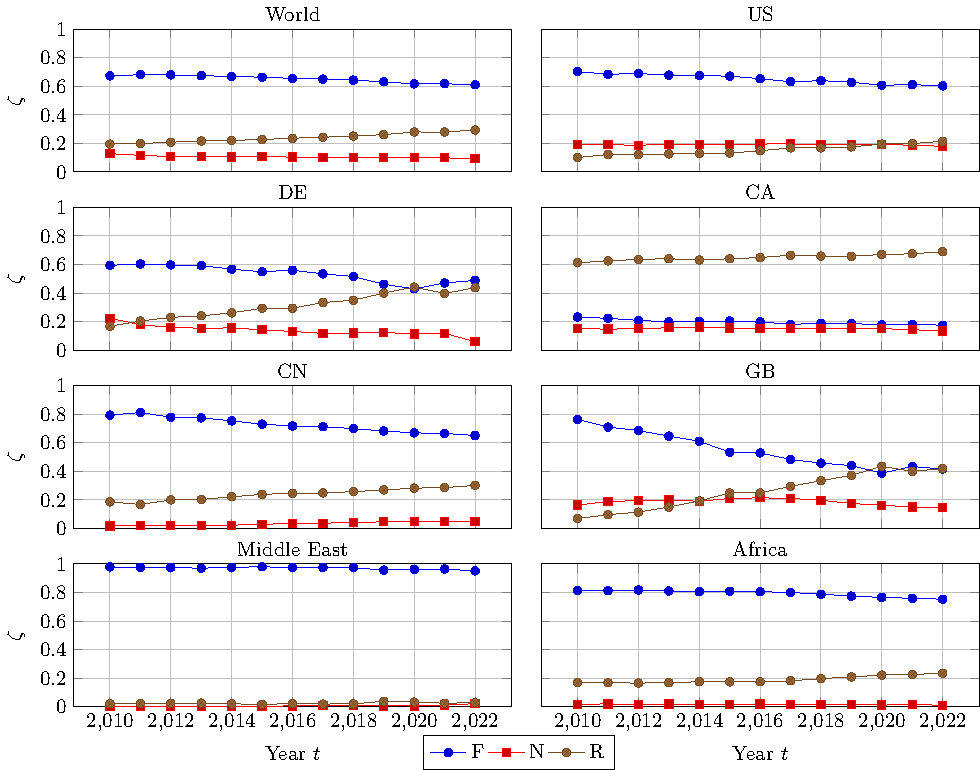
\includegraphics{figures/mix/mix.pdf}
	\caption{Some example countries' and sub-regions' energy mix trends from year 2010 to 2022.}
	\label{fig_mix_data}
\end{figure}

With the observation on the data, we utilize linear regression to model the trend of each energy source's proportion of each country from the data of year 2010 to 2022. Table \ref{table_mix_trend_eqs} shows the results of the linear regression on each of the items.

\begin{table}[!t]
	\centering
	\caption{The linear regression results for the trends of proportion $\zeta$ of energy source over time $t$. The country column represents countries by their ISO 3166-1 alpha-2 codes. For meaningful proportion results, the calculated numerical values of the expressions should be clamped to the range $\left[0, 1\right]$.}
	\label{table_mix_trend_eqs}
	\small
	\begin{tabular}{c|r|r|r}
		\hline
		\textbf{Country} & \textbf{Fossil fuels} $\zeta_{\rm F}$
		& \textbf{Nuclear} $\zeta_{\rm N}$ & \textbf{Renewables} $\zeta_{\rm R}$ \\
		\hline
		AU & $-0.0158t + 32.78$ & 0.00 & $0.0158t - 31.78$ \\
		AT & $-0.0081t + 16.55$ & 0.00 & $0.0079t - 15.16$ \\
		BE & $-0.0086t + 17.59$ & $-0.0060t + 12.59$ & $0.0145t - 29.10$ \\
		CA & $-0.0042t + 8.655$ & $-0.0008t + 1.749$ & $0.0054t - 10.23$ \\
		CL & $-0.0123t + 25.27$ & 0.00 & $0.0124t - 24.56$ \\
		CO & $0.0012t - 2.179$ & 0.00 & $-0.0015t + 3.711$ \\
		CR & $-0.0091t + 18.48$ & 0.00 & $0.0091t - 17.49$ \\
		CZ & $-0.0070t + 14.75$ & $0.0028t - 5.389$ & $0.0041t - 8.118$ \\
		DK & $-0.0415t + 83.98$ & 0.00 & $0.0411t - 82.27$ \\
		EE & $-0.0290t + 59.30$ & 0.00 & $0.0280t - 56.20$ \\
		$\vdots$ &&& \\
		World & $-0.0062t + 13.24$ & $-0.0019t + 4.036$ & $0.0082t - 16.25$ \\
		\hline
	\end{tabular}
\end{table}

According to Equation \ref{eq_dc_emission}, the total annual \ce{CO2} emission of HPC data centers is $\Psi_D = \overline{\rho} T \vb{P}^\top \boldsymbol{\zeta} \vb{M}$ (unless otherwise stated, the values refer to those of year 2024). Therefore, we combine this definition and the constant expanding rate to get
\begin{equation}
	\Psi_D (t) = \overline{\rho} T \left(\vb{P}(t)\right)^\top \boldsymbol{\zeta}(t) \vb{M}
	= \overline{\rho} T r^{t - 2024} \vb{P}^\top \boldsymbol{\zeta}(t) \vb{M},
\end{equation}
where $r = \exp \left(0.1887\right)$ and $\boldsymbol{\zeta}(t)$ is defined in Table \ref{table_mix_trend_eqs}. The calculated numerical values of $\Psi_D(t)$ with $t = 2010, \dots, 2030$ are shown in Figure \ref{fig_datacenter_emission_final}.

To get the \ce{CO2} emissions assuming that 100\% of the electricity is produced from renewable sources, we use $\zeta_{i, \rm F} = 0$, $\zeta_{i, \rm N} = 0$, and $\zeta_{i, \rm R} = 1$ for every country $i$. To get the case of assuming 50\% usage of renewable sources, we do not change the value of $\zeta_{i, \rm N}$ and set $\zeta_{i, \rm F} = 0.5 - \zeta_{i, \rm N}$ and $\zeta_{i, \rm R} = 0.5$ for every country $i$. The results are also shown in Figure \ref{fig_datacenter_emission_final}.

\begin{figure}[!t]
	\centering
	\begin{minipage}{0.48\textwidth}
		\centering
		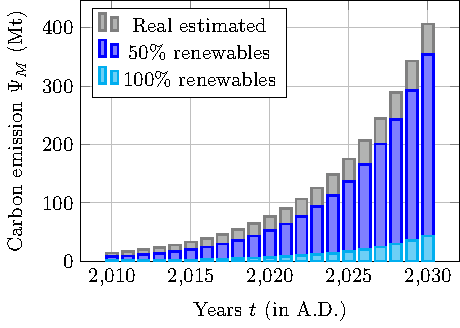
\includegraphics{figures/trends/datacenter_emission.pdf}
		\caption{\ce{CO2} emissions of data centers.}
		\label{fig_datacenter_emission_final}
	\end{minipage}
	\begin{minipage}{0.48\textwidth}
		\centering
		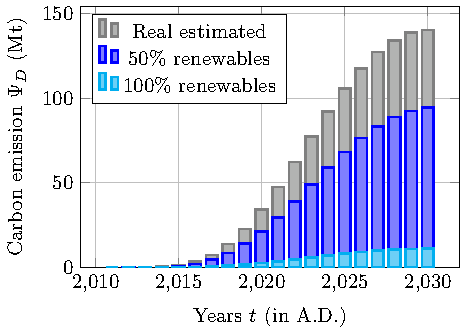
\includegraphics{figures/trends/crypto_emission.pdf}
		\caption{\ce{CO2} emissions of crypto. mining.}
		\label{fig_crypto_emission_final}
	\end{minipage}
\end{figure}

For the change in energy mix of energy used by cryptocurrency, we assume it has a same rate of change as the world's energy mix. With current data of $\zeta_{\rm M, F} = 0.67$, $\zeta_{\rm M, N} = 0.09$ and $\zeta_{\rm M, R} = 0.24$, we have
\begin{equation}
	\begin{aligned}
		\zeta_{\rm M, F}(t) &= -0.0062(t - 2024) + 0.67 = -0.0062t + 13.2188, \\
		\zeta_{\rm M, N}(t) &= -0.0019(t - 2024) + 0.09 = -0.0019t + 3.9356, \\
		\zeta_{\rm M, R}(t) &= 0.0082(t - 2024) + 0.24 = 0.0082t - 16.3568, \\
	\end{aligned}
\end{equation}
and we can calculate the \ce{CO2} emission of cryptocurrency mining as
\begin{equation}
	\Psi_M(t) = \kappa \varepsilon_{\rm opt}(t) H(t) T \boldsymbol{\zeta_M}(t) \vb{M},
\end{equation}
with the numerical results shown in Figure \ref{fig_crypto_emission_final}. Similarly, the cases of having 50\% renewable sources and 100\% renewable are also included.

By adding the values of \ce{CO2} emissions of the two sectors, we have the total \ce{CO2} emissions due to HPC activities $\Psi(t) = \Psi_D(t) + \Psi_M(t)$. The numerical values are shown in Figure \ref{fig_emission_final}.

\begin{figure}[!t]
	\centering
	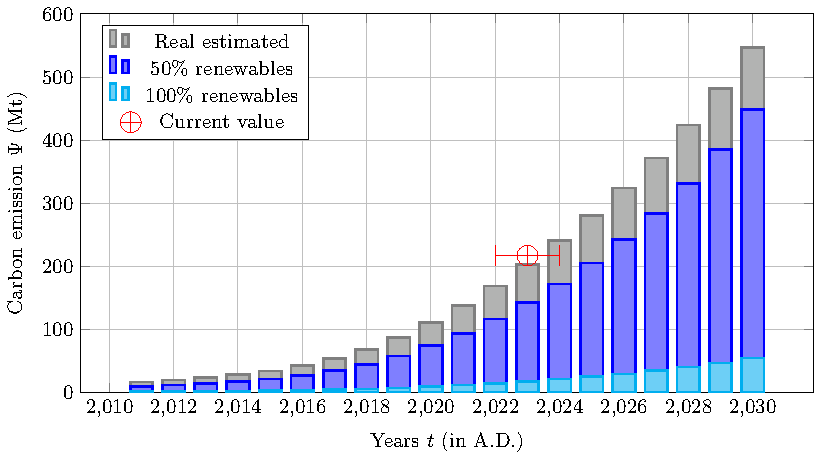
\includegraphics{figures/trends/emission.pdf}
	\caption{Total \ce{CO2} emissions of all HPC activities.}
	\label{fig_emission_final}
\end{figure}

\subsection{Sensitivity analysis}

We conduct sensitivity analysis on the previously valued constants: $\overline{\rho}$, $\kappa$, and $\vb{M}$.

Figure \ref{fig_sens_rho} shows the results of different average HPC data center utilization rates $\overline{\rho}$. With different values tested, there is an obvious positive relationship between $\Psi$ and $\overline{\rho}$. The total carbon emission is very sensitive on the average utilization rate of the data centers since a higher rate means more intensive computing tasks.

\begin{figure}[!t]
	\centering
	\begin{minipage}{0.48\textwidth}
		\centering
		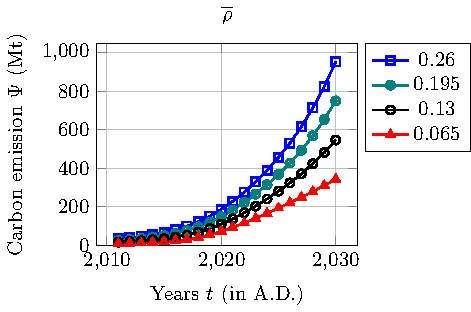
\includegraphics{figures/sensitivity/rho.pdf}
		\caption{Sensitivity analysis: $\overline{\rho}$.}
		\label{fig_sens_rho}
	\end{minipage}
	\begin{minipage}{0.48\textwidth}
		\centering
		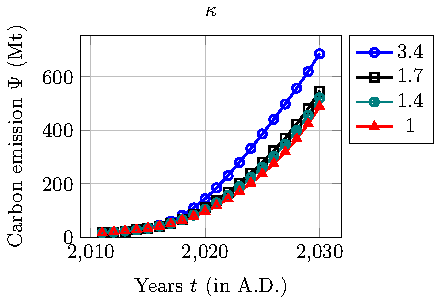
\includegraphics{figures/sensitivity/kappa.pdf}
		\caption{Sensitivity analysis: $\kappa$.}
		\label{fig_sens_kappa}
	\end{minipage}
\end{figure}

Figure \ref{fig_sens_kappa} shows the results of different ratios $\kappa$ between the average and best cryptocurrency mining machines' efficiencies. Note that $\kappa = 1$ is the minimum value possible where all mining machines are up to date with the latest technologies. The changes are not posing very significant differences but still have a relatively strong influence.

A larger ratio indicates a worse overall efficiency, i.e., the devices are mostly older. With the fact of ever-expanding total hash rate, this results in even more devices put into use. Thus, a larger carbon emission is present. The changes are less significant to the total \ce{CO2} emissions due to the larger amount of \ce{CO2} emitted by HPC data centers.

\begin{figure}[!t]
	\centering
	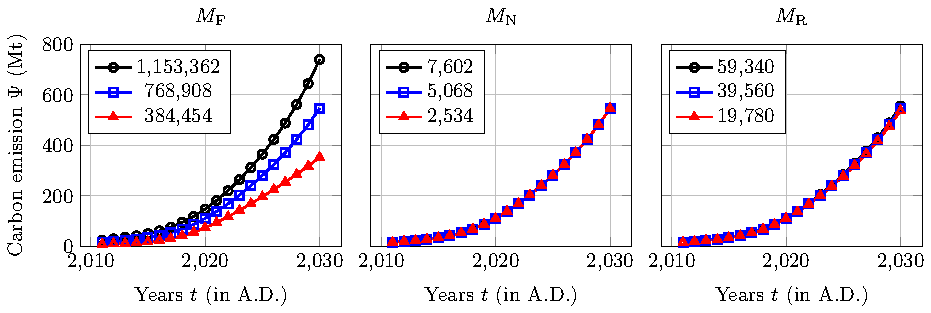
\includegraphics{figures/sensitivity/m.pdf}
	\caption{Sensitivity analysis: $\vb{M}$.}
	\label{fig_sens_m}
\end{figure}

Figure \ref{fig_sens_m} presents the sensitivity analysis on the per-energy \ce{CO2} emission $\vb{M}$, specifically on different energy source types. In reality, such changes are typically because of technology advancements that increase the efficiency of resource uses.

The advancements on fossil fuels have the most significant effects. Since fossil fuels remain to be the most dominant energy type across the world, and it also has the highest per-energy emissions, it contributes most to $\Psi$. The model is very sensitive to changes in $M_{\rm F}$.

On the other hand, for the case of nuclear energy and renewable sources, minimal effects are shown when their \ce{CO2} emissions change. This provides very useful insights on how to reduce total \ce{CO2} emissions through changes in energy mix.

\section{HPC environmental impact model}

In this section, we will devise a comprehensive model to determine a qualitative impactfulness of HPC activities. We will make use of the aforementioned calculated data as well as a new model regarding water consumption that will be developed.

\subsection{Impact of carbon dioxide emissions}

The negative effect of \ce{CO2} emission is its consequential aggravation on global warming, which is presented through the increase in average global temperature.

There is a logarithmic relationship between the temperature change $\Delta T$ and the change in \ce{CO2} concentration $\Delta C$ \citep{co2emission_log}, defined as
\begin{equation}
	\Delta T = S \ln \left(\frac{C_0 + \Delta C}{C_0}\right) \rm (^\circ C),
\end{equation}
where $S$ is a constant and $C_0$ is the reference concentration (typically the present level).

Researches have found that the constant $S \approx 3.42 \rm ^\circ C$ \citep{co2conc_warming_relationship}. According to data from NASA Global Climate Change, the current \ce{CO2} concentration in atmosphere is $C_0 = 422 \rm ppm$ \citep{co2conc}. This correlation is depicted in Figure \ref{fig_co2conc_temp}. It is reasonable to assume $C_0$ constant since the formula calculates the warming effects from a proportional change in concentration and the $\Delta C$ is negligible compared with the overall atmosphere.

\begin{figure}[!b]
	\centering
	\begin{minipage}{0.48\textwidth}
		\centering
		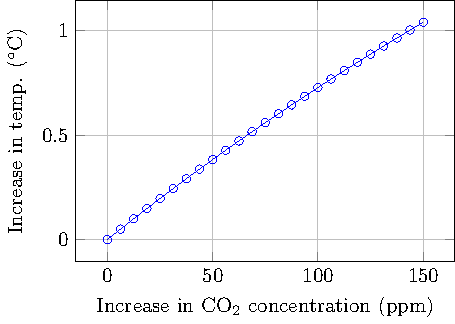
\includegraphics{figures/impact/conc_temp.pdf}
		\caption{The relationship (at $C_0 = 422 \rm ppm$) between the increase in \ce{CO2} concentration and the increase in average global temperature.}
		\label{fig_co2conc_temp}
	\end{minipage}
	\hfill
	\begin{minipage}{0.48\textwidth}
		\centering
		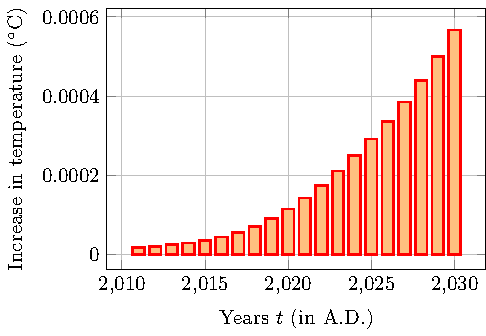
\includegraphics{figures/impact/temperature.pdf}
		\caption{The estimated annual global temperature increment by year from 2010 to 2030, calculated from carbon emission data.}
		\label{fig_temperature}
	\end{minipage}
\end{figure}

The mass of the atmosphere is approximately $5.148 \times 10^{9} \rm Mt$ \citep{atmosphere_mass}. Therefore, the \ce{CO2} emission, considering the molar mass of \ce{CO2}, $44.01 \rm g/mol$, and the atmosphere, $28.97 \rm g/mol$, would contribute an additional
\begin{equation}
	\frac{\Delta C}{m} = \frac{n_{\rm air}}{n_{\ce{CO2}}} \cdot 10^6
	= \rm \frac{\sfrac{1Mt}{(44.01 g/mol)}}{\sfrac{(5.148 \times 10^9 Mt)}{(28.97 g/mol)}} \times 10^6
	= 1.279 \times 10^{-4} ppm/Mt
\end{equation}
increase to the \ce{CO2} concentration. Hence, the increase in global temperature due to \ce{CO2} emission from HPC can be modeled as
\begin{equation}
	\Delta T = S \ln \left(\frac{C_0 + \Psi \cdot \frac{\Delta C}{m}}{C_0}\right)
	= 3.42 \cdot \ln \left(\frac{422 + 1.279 \times 10^{-4} \cdot \Psi}{422}\right) \rm (^\circ C),
\end{equation}
where $\Psi$ is the carbon emission of HPC, in megatons (Mt). Using data in previous models, we can calculate the numerical results of the global temperature increase due to HPC's \ce{CO2} emissions in each year, as shown in Figure \ref{fig_temperature}.

According to NOAA's 2023 Annual Climate Report \citep{temperature}, the world currently has an average temperature increase rate of $0.02 \rm ^\circ C$ per year and an average temperature $1.35 \rm ^\circ C$ higher than pre-industrial average.

To indicate whether the contribution to global warming is in a reasonable range, i.e. \textit{how high is too high}, as a \textit{qualitative} measure, we consider a threshold ratio $r = \Delta T_{i + 1} / \Delta T_i \in (0, 1)$ of the temperature increment between two years. $r$ is defined as that with such a ratio no larger than $r$, it would be possible to keep the world temperature increment (from pre-industrial average) under a certain temperature $T$ perpetually, namely
\begin{equation}
	\left\{T_i\right\} = 0.02 \cdot r^{i - 2023}, \quad
	\sum_{i = 2023}^\infty T_i = \frac{0.02}{1 - r} = T - 1.35.
\end{equation}

Using $T = 1.5 \rm ^\circ C$ and $T = 2 \rm ^\circ C$ (as proposed in the Paris Agreement), we can solve for $r$, yielding $r = 0.87$ and $r = 0.97$, respectively. We define \textit{good} as the annual temperature increment able to keep the change below $1.5 \rm ^\circ C$, \textit{intermediate} as between $1.5 \rm ^\circ C$ and $2 \rm ^\circ C$, and \textit{bad} as above $2 \rm ^\circ C$.

\begin{figure}[!b]
	\centering
	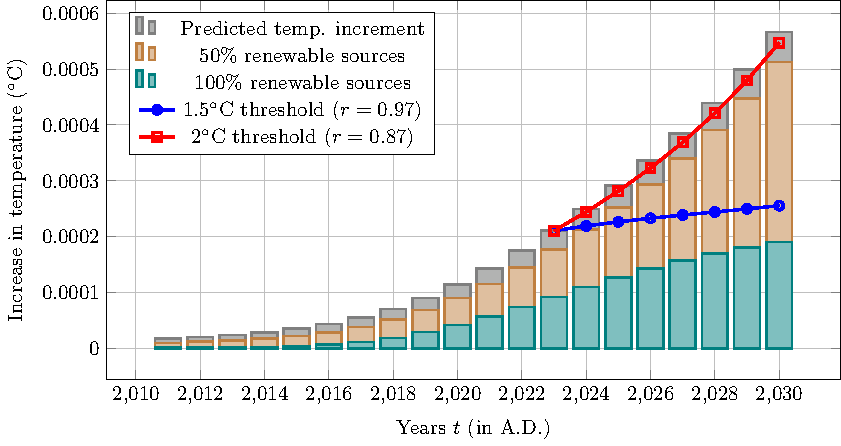
\includegraphics{figures/impact/temp_i.pdf}
	\caption{The global warming effects of the predicted developments and cases of using 50\% and 100\% energy from renewable sources. The threshold values to achieve $T = 1.5 \rm ^\circ C$ and $T = 2 \rm ^\circ C$ are also included; note that they only offer the rough boundaries of a qualitative analysis.}
	\label{fig_warming_final}
\end{figure}

We use the data of temperature increase due to HPC in year 2023 as a reference and create a consequential trend of \textit{threshold} annual increments with ratio $r$ and the rate of expansion of HPC. We then define, for a specific year, if the annual increment in temperature is below the trend, then that year will be considered to be able to achieve the temperature goal of $T$. This is reasonable as a \textit{qualitative measure}:
\begin{enumerate}
	\item If a specific annual increment exceeds the trend, then it will require a more intense decrease than $r$ in the following years to reach the temperature target, vice versa;
	\item HPC is not likely to take a disproportionally high share of all industries, and thus it is reasonable to use the year 2023's data as the reference and indicate whether it will be burdening the world;
	\item The measure is not subdivided (with only three states), and a rough estimation is enough.
\end{enumerate}

We plot the temperature impacts for the estimated values and the threshold values, as well as the case of using 50\% and 100\% renewable energy sources, in Figure \ref{fig_warming_final}. 

\subsection{New factor: impact of water consumption}

While global warming is a great concern and is the most obvious environmental cost of HPC, its water consumption is also tremendous and cannot be ignored.

Therefore, considering the crisis of scarcity of fresh water in many regions, \textbf{water usage} is selected as another significant environmental concern of HPC. The reasons for choosing it are as follows:
\begin{enumerate}
	\item As addressed above, the scarcity of fresh water is a severe global issue;
	\item Compared with factors like land use and resource depletion, since there is always increasing demand for HPC that cannot be ignored, modeling water usage is more practical for the easier actionability to reduce the negative effects;
	\item This water usage model can be a foundation for further expansions of the model to more factors, such as chemical use (which is mostly related to cooling systems too) and land use (for better water availability or alternative environmental cooling methods).
\end{enumerate}

Water consumption is directly related to power consumption since it is used for cooling. The global average water consumption of server clusters is 1.8 liters per kilowatt-hour \citep{water_efficiency}, which directly converts to 1.8Mt/TWh. Therefore, the total water consumption can be calculated as
\begin{equation}
	W(t) = 1.8 E(t),
\end{equation}
where $E$ is the total energy consumption of HPC.

\begin{figure}[!t]
	\centering
	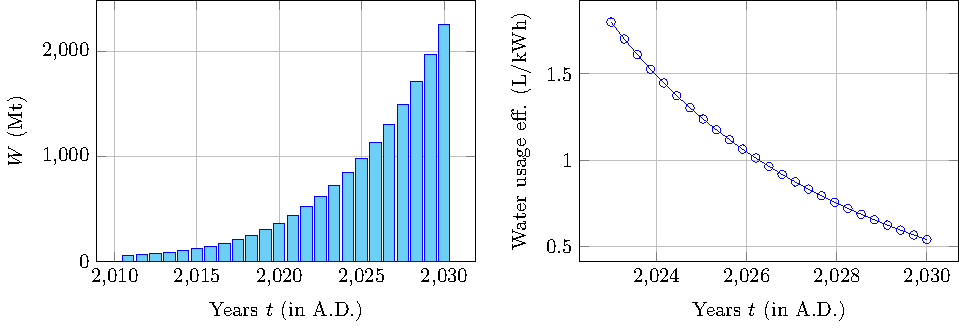
\includegraphics{figures/water/water.pdf}
	\caption{Water consumption data. \textbf{Left:} The trend of total water consumption due to HPC. \textbf{Right:} The required water usage effectiveness to maintain current level of water usage.}
	\label{fig_water}
\end{figure}

Figure \ref{fig_water} (left) presents the data, where about 679Mt water is consumed by HPC in the year of 2023. We can see that there is a very rapid growth of water demand, with the year 2030 exceeding 2,000Mt, if assumed constant water usage effectiveness.

Modeling the trend of water usage effectiveness over time remains to be a challenge. However, we can calculate the values required to maintain the current level of water consumption. This can also be very useful to offer insights for a reference on technological development, without having the exact knowledge of the trend.

\section{Result sharing and discussions}

\subsection{Recommendations to reduce the environmental impacts}

Based on the results of our final HPC environmental impact model, we can propose recommendations to reduce the negative environmental impacts as follows.

\subsubsection{To policymakers}

A change in energy mix would be very helpful. Governments may set up taxes on carbon emission and subsidies on the use of renewable energies to firms. This will provide price incentives for the firms to switch their energy mix. Regulations and legislations on HPC firms and cryptocurrency miners should also be imposed. There could be periodic mandatory reviews on these sites to control their energy and water usages.

An example of the effects in our model is shown in Figure \ref{fig_warming_final} as part of the model results. From the plot, we can see that a slight increase in the porportion of renewable sources would be enough to achieve the long-term goal of under $2 \rm ^\circ C$ temperature increase; if the policy is effective enough to push the porportion above 50\% before 2026, the goal of $1.5 \rm ^\circ C$ can also be achieved.

\subsubsection{To tech companies and cryptocurrency miners}

The current server utilization rate is low. In the future, when trying to expand the overall computing power, consider increasing the utilization of resources before directly expanding the number of devices. Containerization technologies can be applied to make use of the unemployed resources.

Switching to cooling systems that recirculate water can significantly reduce the amount of fresh water consumed. It could also be beneficial to collect rain water or use recycled water.

Self-built solar power would also be a good option. Since they require almost zero operational cost once installed, it would be more cost-efficient and greener.

\subsection{Discussions on our models}

\subsubsection{Strengths}

\textbf{Accurate.} We use comprehensive and detailed real-world data to predict the trends in the following decade. \textbf{Interpretable.} We have a very clear division of subtasks, each of which follows a mathematically interpretable small model. \textbf{Extensible.} Our careful design of splitting HPC into sectors and calculating country-wise data and trends is to ensure that the model can be easily extended when more data are available. \textbf{Objective.} There is barely subjective intuitions involved in the development of the model, and all trends are strongly data-driven.

\subsubsection{Weaknesses}

\textbf{Partial impacts included.} Among various environmental factors of HPC, we only used two of them (energy consumption and water usage). \textbf{Possible oversimplification.} We have ignored many scenarios and minor factors that may also contribute to the trends. \textbf{Possibly uncomprehensive.} Throughout the model, we are only calculating the effects and data during HPC operations, while excluding phases like construction and hardware renewing; in reality, these all account for the environmental impacts.

\newpage

\begin{center}
	\section{A letter to the United Nations Advisory Board}
\end{center}

\bigskip
Dear United Nations Advisory Board,
\bigskip
\bigskip

This is HiMCM Team 15803, and we are writing this letter to you in response to your recent report \textit{Governing AI for humanity} in which we believe the environmental impact of high-powered computing (HPC) is in absence.

While the report detailedly outlines the strategies and ethical considerations of AI development, we are concerned that the growing environmental impact of HPC on our planet was not fully discussed. This is also a great challenge for humanity. The training process of AI models is part of the HPC activities. With the rising popularity of large language models in recent years, more and more tech companies are involved in this endless competition, leading to a vast expansion of the HPC industry.

The expansion of HPC is never a small thing. Having more HPC hosts means having more and more server clusters intensively operating 24 hours a day, 7 days a week around the world. We developed the HPC Environmental Impact Model to investigate the impacts of the currently growing trend of HPC and found that, if without proper interventions, the industry would grow in a tremendous rate and create irreversible damages to our planet Earth. By the year of 2030, it would consume more than two times the energy and emit almost three times the amount of \ce{CO2} than it currently does.

This will lead to the exponentially growing global warming effects. If no measures are taken, then the prospective plan of controlling the global temperature increase under $1.5 \rm ^\circ C$ above pre-industrial level will soon be broken by the growth of HPC. Moreover, there will also be two times the water consumption than now, reaching over 2 billion tons of water, to be directly occupied by HPC every year. This will further intensify the current water scarcity problem.

Therefore, we strongly urge you to add the concerns regarding HPC to the 2030 developmental goals, to align with the principles of sustainable development. We think that it would be important to have an energy mix standard for all HPC energy supplies, at the level of at least 50\% from renewable sources by 2030, according to our model. There should also be transparent carbon footprint and water consumption reporting specifically for HPC activities in each country.

We believe that the United Nations should take the responsibility of incentivizing countries for a better energy mix and fight for our collective well-being.

We believe that the severity of this issue is not lower than the ethical issues of AI; instead, we think that this should be of the highest priority among all AI issues. This is a direct threat to our nature, our planet Earth, and everyone's well-being.

We appreciate your efforts on shaping more responsible AI, and we are glad if we can have further contribution to this crucial topic.

Thanks for your time and consideration on this matter.

\bigskip
\bigskip
\hfill Sincerely,

\hfill HiMCM Team 15803

\newpage

\let\Section\section 
\def\section*#1{\Section{#1}}
\bibliographystyle{apalike}
\bibliography{bib.bib}

\end{document}